\documentclass[11pt,a4paper]{report}
\usepackage[T1]{fontenc}
\usepackage[utf8]{inputenc}
\usepackage[a4paper,margin=2.6cm]{geometry}
\usepackage{amssymb}
\usepackage{mathptmx}
\usepackage[scaled=.92]{helvet}
\usepackage{courier}
\usepackage{microtype}
\usepackage{xcolor}
\usepackage{booktabs,longtable,array}
\usepackage{enumitem}
\usepackage{fancyhdr}
\usepackage{titlesec}
\usepackage{tikz}
\usetikzlibrary{positioning,arrows.meta,shapes.geometric,fit,backgrounds}
\usepackage{listings}
\usepackage[most]{tcolorbox}
\usepackage[hidelinks]{hyperref}
\usepackage{url}
\urlstyle{tt}
\Urlmuskip=0mu plus 2mu
\def\UrlBreaks{\do\.\do\_\do\/\do\-\do\(\do\,}
\emergencystretch=3em

\definecolor{accent}{HTML}{FF5A1F}
\definecolor{ink}{HTML}{222222}
\definecolor{muted}{HTML}{6B6B6B}
\definecolor{codebg}{HTML}{F6F6F4}
\definecolor{kw}{HTML}{1F5FA8}
\definecolor{cm}{HTML}{6A7F6A}
\definecolor{st}{HTML}{B5441A}

\setlist{itemsep=2pt,topsep=4pt}
\setlength{\parindent}{0pt}
\setlength{\parskip}{6pt}

\titleformat{\chapter}[hang]{\sffamily\Huge\bfseries\color{ink}}{\color{accent}\thechapter}{.5em}{}
\titlespacing*{\chapter}{0pt}{-10pt}{22pt}
\titleformat{\section}{\sffamily\Large\bfseries\color{ink}}{\color{accent}\thesection}{.5em}{}
\titleformat{\subsection}{\sffamily\large\bfseries\color{ink}}{\thesubsection}{.5em}{}

\pagestyle{fancy}
\fancyhf{}
\fancyhead[L]{\small\color{muted}BikeTools Analyzer --- Developer guide}
\fancyhead[R]{\small\color{muted}\leftmark}
\fancyfoot[C]{\small\thepage}
\renewcommand{\headrulewidth}{0.3pt}
\renewcommand{\chaptermark}[1]{\markboth{#1}{}}
\fancypagestyle{plain}{\fancyhf{}\fancyfoot[C]{\small\thepage}\renewcommand{\headrulewidth}{0pt}}

% inline code: breakable, underscores allowed (do not use # or % inside)
\newcommand{\code}[1]{\nolinkurl{#1}}

\lstdefinestyle{py}{
  language=Python, basicstyle=\ttfamily\footnotesize, backgroundcolor=\color{codebg},
  keywordstyle=\color{kw}\bfseries, commentstyle=\color{cm}\itshape, stringstyle=\color{st},
  frame=single, rulecolor=\color{codebg}, framesep=5pt, xleftmargin=5pt, xrightmargin=5pt,
  breaklines=true, breakatwhitespace=false, showstringspaces=false, columns=fullflexible,
  aboveskip=8pt, belowskip=6pt, upquote=true, keepspaces=true
}
\lstdefinestyle{plain}{
  basicstyle=\ttfamily\footnotesize, backgroundcolor=\color{codebg}, frame=single, rulecolor=\color{codebg},
  framesep=5pt, xleftmargin=5pt, xrightmargin=5pt, breaklines=true, columns=fullflexible,
  aboveskip=8pt, belowskip=6pt, showstringspaces=false, keepspaces=true
}
\lstset{style=py}
\newcommand{\shell}[1]{\lstset{style=plain}#1\lstset{style=py}}

\newtcolorbox{tip}[1][Tip]{enhanced,breakable,colback=accent!6,colframe=accent,boxrule=0pt,
  leftrule=3pt,arc=0pt,left=8pt,title=#1,fonttitle=\bfseries\small,coltitle=ink,
  colbacktitle=accent!6,attach boxed title to top left={yshift=-2mm},boxed title style={size=small}}
\newtcolorbox{warn}[1][Pitfall]{enhanced,breakable,colback=red!4,colframe=red!60!black,boxrule=0pt,
  leftrule=3pt,arc=0pt,left=8pt,title=#1,fonttitle=\bfseries\small,coltitle=ink,
  colbacktitle=red!4,attach boxed title to top left={yshift=-2mm},boxed title style={size=small}}

\newcommand{\checklist}[1]{\begin{itemize}[label=$\square$]#1\end{itemize}}

\begin{document}

\begin{titlepage}
\raggedright
\vspace*{3cm}
{\color{accent}\rule{3cm}{4pt}}\\[1.2cm]
{\Huge\bfseries BikeTools Analyzer}\\[.4cm]
{\LARGE Developer guide}\\[1.2cm]
{\large How the code is organised and how to extend it:\\
new metrics, charts, file formats, services and pages.}\\[3cm]
{\color{muted}Repository \texttt{jplanari/BikeToolsAnalyzer}\\
Applies to the app version shown in the page header (v1.4) and the database
metrics version 6.}
\vfill
{\small\color{muted}This guide describes the code as it is in the repository. When it and the code disagree, the code wins;
please fix the guide in the same pull request.}
\end{titlepage}

\tableofcontents

\chapter{Introduction}

BikeTools Analyzer is a Streamlit application that reads cycling activities (FIT, GPX, TCX, or straight from Strava,
Wahoo and Polar), stores them in a local SQLite database and turns them into ride analysis, training-load analytics,
physics-based models (aerodynamics, climbing, thermal) and PDF reports. It runs on a rider's own computer, either with
\texttt{streamlit run} or as a packaged desktop program. All data stays on that computer.

The project is meant to be changed by the people who use it. This guide exists so that a change does not need a
long reading session first: it explains the few ideas the whole code base is built on, then gives step-by-step
recipes for the changes people most often want.

\section*{What you can add, and where to look}

\begin{center}
\small
\begin{tabular}{@{}p{5.4cm}p{3.3cm}p{5.2cm}@{}}
\toprule
I want to\ldots & Read & Touches mostly\\
\midrule
add a per-ride number (metric) & \S\ref{rec:metric} & \code{analysis/}, \code{pipeline.py}, \code{db.py}\\
add an analysis to the Training page & \S\ref{rec:training} & \code{analysis/}, \code{viz/training_page.py}\\
add a section to the ride page & \S\ref{rec:ridesection} & \code{viz/ride_analysis.py}\\
add a chart & \S\ref{rec:plot} & \code{viz/plots.py}, \code{training_plots.py}\\
read a new file format & \S\ref{rec:format} & \code{data/}, \code{pipeline.py}\\
connect a new online service & Chapter~\ref{ch:providers} & \code{data/}, \code{viz/sidebar.py}\\
add a profile setting & \S\ref{rec:setting} & \code{db.py}, \code{viz/user_corner.py}\\
add something to the PDF report & \S\ref{rec:report} & \code{report_data.py}, \code{report_pdf.py}\\
change the look & \S\ref{sec:theme} & \code{viz/theme.py}\\
\bottomrule
\end{tabular}
\end{center}

\section*{Three rules that make changes safe}

\begin{enumerate}
\item \textbf{Calculations never touch the screen.} Everything under \code{src/analysis}, \code{src/physics} and
  \code{src/data} is plain Python on pandas objects, with no Streamlit calls. That is what makes it testable and
  reusable by the PDF report. (A few data modules still import Streamlit for caching; see \S\ref{sec:headless}.)
\item \textbf{The original file is the source of truth.} Every ride's file is stored, so any metric can be
  recomputed later. A new metric therefore never needs the rider to re-upload anything.
\item \textbf{Add a test with the change.} The test suite is quick (under a minute) and runs on every push.
  Chapter~\ref{ch:conventions} lists what to test.
\end{enumerate}

\chapter{Getting started}

\section{Run it from source}

You need Python 3.10 or newer (the continuous-integration build uses 3.11).

\begin{lstlisting}[style=plain]
git clone https://github.com/jplanari/BikeToolsAnalyzer
cd BikeToolsAnalyzer
python -m venv .venv
.venv\Scripts\activate          # Windows;  macOS/Linux: source .venv/bin/activate
pip install -r requirements.txt
streamlit run app.py --server.port 8501
\end{lstlisting}

Port 8501 matters: the Strava, Wahoo and Polar sign-in redirects point at \code{http://localhost:8501/}. If another
program holds it, Streamlit silently moves to 8502 and sign-in breaks.

The database file is \texttt{bikethools.db} in the folder you start from (the spelling is historical). Set the
environment variable \code{BIKETOOLS_DB} to keep it elsewhere, for example outside a OneDrive or Dropbox folder,
whose sync clients lock files in ways SQLite dislikes. The desktop build uses its own per-user data folder.

\begin{tip}[Use a scratch database while developing]
\begin{lstlisting}[style=plain]
set BIKETOOLS_DB=C:\temp\dev.db          # Windows (cmd)
$env:BIKETOOLS_DB="C:\temp\dev.db"       # Windows (PowerShell)
export BIKETOOLS_DB=/tmp/dev.db          # macOS / Linux
\end{lstlisting}
Your real rides stay untouched while you experiment.
\end{tip}

\section{Run the tests}

\begin{lstlisting}[style=plain]
pytest                       # everything
pytest tests/test_upload.py  # one file
pytest -k thresholds -q      # by name
\end{lstlisting}

Continuous integration (\code{.github/workflows/python-app.yml}) installs \texttt{requirements.txt}, then runs
\texttt{pytest} on every push. Two kinds of test exist:

\begin{itemize}
\item \textbf{Headless tests} (most of them) import the calculation and data modules directly. If a heavy library is
  missing on your machine, \code{tests/conftest.py} replaces it with a stub, so these tests still run.
\item \textbf{User-interface tests} (\code{tests/test_ui.py}, \code{tests/test_training_page.py}) start the real
  application with Streamlit's \texttt{AppTest}, click through the pages against a seeded database, and fail on any
  exception. They are skipped locally when Streamlit is not installed, but \emph{required} in CI.
\end{itemize}

\section{Make a change}

\begin{enumerate}
\item Create a branch from \texttt{main}: \texttt{git checkout -b my-feature}.
\item Make the change and its tests; run \texttt{pytest}.
\item Push and open a pull request. CI runs the same tests.
\item To try it as the desktop app, run the \emph{Desktop build} workflow (Actions tab) on your branch.
\end{enumerate}

Keep pull requests focused. A new metric, a new chart and a new service are three pull requests, not one; each is
then easy to review and to revert.

\chapter{Architecture}

\section{Layers}

The code is four layers. A module may import from the layers to its right, never from the left.

\begin{center}
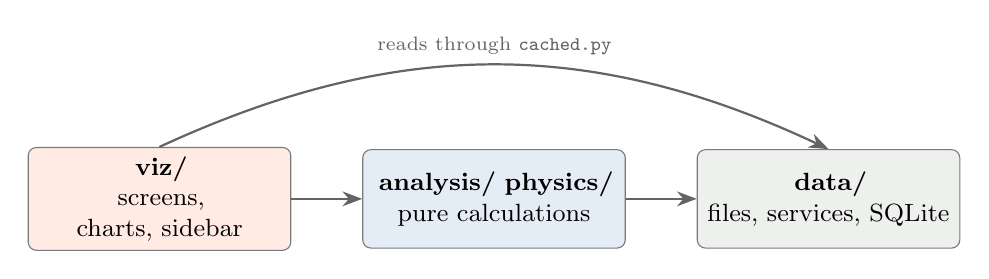
\begin{tikzpicture}[
  box/.style={rectangle,rounded corners=3pt,draw=ink!60,fill=#1!12,minimum height=1.25cm,text width=3.1cm,align=center,font=\small},
  arr/.style={-{Stealth[length=2.5mm]},thick,ink!70}]
\node[box=accent] (viz) {\textbf{viz/}\\screens, charts, sidebar};
\node[box=kw,right=0.9cm of viz] (analysis) {\textbf{analysis/ physics/}\\pure calculations};
\node[box=cm,right=0.9cm of analysis] (data) {\textbf{data/}\\files, services, SQLite};
\draw[arr] (viz) -- (analysis);
\draw[arr] (analysis) -- (data);
\draw[arr,bend left=25] (viz.north) to node[above,font=\scriptsize]{reads through \texttt{cached.py}} (data.north);
\end{tikzpicture}
\end{center}

\begin{description}[style=nextline,leftmargin=1.2em]
\item[\code{src/data}] Everything that is read or written: file parsers (\code{fit.py}, \code{gpx.py}, \code{tcx.py}),
  service clients (\code{strava.py}, \code{wahoo.py}, \code{polar.py}), the SQLite layer (\code{db.py}) and the
  \emph{pipeline} (\code{pipeline.py}) that turns a file into a standard table and its summary numbers.
\item[\code{src/analysis}] Pure functions: normalized power and TSS (\code{power.py}), per-ride quality metrics
  (\code{ride_metrics.py}), the performance management chart (\code{training_load.py}), power profile and critical
  power (\code{power_profile.py}), climbs, segments, correlations, workout building.
\item[\code{src/physics}] Models of the rider and the road: aerodynamic drag and CdA (\code{aerodyn.py}), a climbing
  model (\code{climb_model.py}), heat balance (\code{thermal.py}).
\item[\code{src/viz}] Everything with Streamlit or Plotly in it: the page for each mode, the sidebar, charts, the
  look, and the PDF writers.
\end{description}

The entry point is \code{app.py}. It initialises the database, applies the look, finishes any pending sign-in
redirect, draws the sidebar, then draws one of three pages according to the top navigation bar.

\section{Repository map}

\begin{longtable}{@{}p{5.6cm}p{9.3cm}@{}}
\toprule
Path & Role\\
\midrule
\endhead
\code{app.py} & Entry point; chooses the page.\\
\code{src/viz/sidebar.py} & Users, data sources (upload, Strava, Wahoo, Polar), sign-in callbacks.\\
\code{src/viz/ride_analysis.py} & The ride page: parse, summarise, save, then draw sections.\\
\code{src/viz/training_page.py} & The Training page (load, power profile, durability, intensity, deeper).\\
\code{src/viz/user_corner.py} & Profile, thresholds, history repair, Connections form.\\
\code{src/viz/connections.py} & In-app entry of service credentials.\\
\code{src/viz/plots.py}, \code{training_plots.py} & Plotly chart builders.\\
\code{src/viz/figstyle.py} & Keeps chart titles and legends from overlapping (automatic).\\
\code{src/viz/sections.py} & Tab-like selector and \texttt{remembered()} widgets.\\
\code{src/viz/theme.py} & Look (CSS), welcome page, help texts.\\
\code{src/viz/report_pdf.py}, \code{ride_report_pdf.py} & PDF writers (matplotlib).\\
\code{src/data/pipeline.py} & File $\rightarrow$ standard table $\rightarrow$ summary dict.\\
\code{src/data/db.py} & Schema, migrations, every read and write.\\
\code{src/data/cached.py} & Cached reads for the pages.\\
\code{src/data/credentials.py} & Where service client IDs and secrets come from.\\
\code{src/data/*_import.py} & Import workflows per source.\\
\code{src/data/thresholds.py} & FTP and LTHR estimated from data.\\
\code{desktop/} & Launcher and PyInstaller recipe for the packaged app.\\
\code{docs/} & OAuth forwarding page, physics report, this guide.\\
\code{tests/} & One test file per area.\\
\bottomrule
\end{longtable}

\section{How a ride travels through the app}

\begin{center}
\begin{tikzpicture}[
  node distance=0.55cm,
  s/.style={rectangle,rounded corners=3pt,draw=ink!60,fill=codebg,minimum height=0.9cm,text width=11.5cm,align=left,font=\small},
  arr/.style={-{Stealth[length=2mm]},ink!70}]
\node[s] (a) {\textbf{1. Source.} Upload, Strava, Wahoo or Polar delivers file bytes and a file name.};
\node[s,below=of a] (b) {\textbf{2. \code{prepare_ride}} (\code{pipeline.py}). Detect the format from content, parse, clean impossible
  readings, resample to 1\,Hz, add distance, speed and grade. Result: one \texttt{DataFrame}.};
\node[s,below=of b] (c) {\textbf{3. \code{summarize_ride}.} Normalized power, TSS, zones, power curve, decoupling, \ldots\ in one dict.};
\node[s,below=of c] (d) {\textbf{4. \code{db.save_ride}.} Metadata, power curve, zone times, histograms \emph{and the original file} are stored.};
\node[s,below=of d] (e) {\textbf{5. Pages.} Training analytics read the stored numbers, never the files. The ride page works on the DataFrame.};
\foreach \x/\y in {a/b,b/c,c/d,d/e} \draw[arr] (\x) -- (\y);
\end{tikzpicture}
\end{center}

Stored numbers make the Training page fast: it reads rows, it does not re-parse hundreds of files. The ride page,
which needs second-by-second data, works on the DataFrame from step 2.

\chapter{The data model}

\section{The standard ride table}

\code{prepare_ride(filename, file_bytes)} returns \code{(df, total_dist_m, total_ascent_m)}. The DataFrame has one
row per second and these columns (a column is absent or all-\texttt{NaN} when the device did not record it):

\begin{center}
\small
\begin{tabular}{@{}lll@{}}
\toprule
Column & Meaning & Unit\\
\midrule
\texttt{time} & timestamp (naive, UTC) & datetime\\
\texttt{lat}, \texttt{lon}, \texttt{ele} & position and elevation & degrees, m\\
\texttt{power}, \texttt{hr}, \texttt{cadence} & sensor values & W, bpm, rpm\\
\texttt{speed} & ground speed & m/s\\
\code{dist_m} & cumulative distance & m\\
\texttt{grade}, \code{grade_smooth} & road gradient & \%\\
\code{temp_c} & device temperature (FIT only) & $^\circ$C\\
\texttt{bearing} & direction of travel (added by the ride page) & degrees\\
\bottomrule
\end{tabular}
\end{center}

\begin{warn}
\texttt{speed} is in \emph{metres per second}; a convenience column \code{speed_kmh} also exists. Mixing the two is
the most common source of wrong numbers. Convert at the edge, on display.
\end{warn}

Always test for a channel before using it:

\begin{lstlisting}
has_power = 'power' in df.columns and df['power'].notna().any()
\end{lstlisting}

Indoor rides have no GPS, runs on the same watch have no power, cheap sensors have no cadence; every analysis must
degrade gracefully, never raise.

\section{Cleaning}

\code{clean_channels} (in \code{cleaning.py}) runs before any metric. It removes physically impossible readings: power
above 2500\,W or negative, heart rate outside 30--230\,bpm, cadence above 220\,rpm. Short power glitches are
interpolated; longer ones become 0\,W. The number of samples changed is kept in \texttt{df.attrs['cleaned']}.
If you add a sensor channel, add its sanity limits there so that one bad sample cannot become a record.

\section{The summary dictionary}

\code{summarize_ride(df, ftp, lthr)} returns the dictionary the ride page shows and the database stores:

\begin{center}
\small
\begin{tabular}{@{}p{3.6cm}p{10.6cm}@{}}
\toprule
Key & Content\\
\midrule
\code{duration_s}, \code{moving_time_s} & elapsed seconds; seconds with speed $\geq$ 2\,m/s (or pedalling, if no speed)\\
\code{avg_speed_kph}, \code{avg_power}, \code{avg_hr} & averages over moving time\\
\code{norm_power}, \texttt{if}, \texttt{tss}, \code{tss_source} & load; \code{tss_source} says whether it came from power or heart rate\\
\texttt{kj}, \texttt{vi}, \texttt{ef}, \code{decoupling_pct} & work, variability index, efficiency factor, aerobic decoupling\\
\code{power_curve} & mean-maximal power per duration, \texttt{\{seconds: watts\}}\\
\texttt{zones} & seconds per zone: \texttt{\{'power': \{...\}, 'hr': \{...\}\}}\\
\texttt{fatigued} & power curves of the part of the ride after 1000, 2000 and 3000\,kJ of work (durability)\\
\texttt{hist} & joint histograms power$\times$HR and power$\times$cadence\\
\texttt{hrr60}, \code{hrr_efforts}, \texttt{hr20} & heart-rate recovery; best 20-minute heart rate\\
\code{is_moving} & boolean mask over the rows of \texttt{df}\\
\bottomrule
\end{tabular}
\end{center}

\code{metrics_for_storage(summary)} selects the keys that go to the database. Note the two places where a key is
renamed on the way in (\code{moving_time_s} $\to$ column \code{moving_s}, \texttt{hrr60} $\to$
\code{hrr60_bpm}); the mapping lives in \code{db._metrics_fields}.

\section{The database}

SQLite, one file, opened through \code{db._connect()} only (it turns on foreign keys, so deleting a user cascades to
their rides). The schema is created by \code{init_db()} and extended by \code{migrate_db()}.

\begin{center}
\small
\begin{tabular}{@{}p{3.5cm}p{11.2cm}@{}}
\toprule
Table & Holds\\
\midrule
\texttt{users} & name, FTP, LTHR, weight, height, CP, W$'$, crank length; \code{ftp_auto}/\code{lthr_auto} flags\\
\texttt{rides} & one row per ride: date, distance, NP, TSS, IF, VI, EF, \ldots, \code{metrics_version}\\
\code{ride_files} & the original file, compressed (\texttt{codec}, \texttt{content})\\
\code{power_records} & the ride's power curve, one row per duration\\
\code{power_records_kj} & the same after a given amount of work\\
\code{ride_zones} & seconds per zone and kind (\texttt{power}, \texttt{hr})\\
\code{ride_hist} & sparse 2-D histogram cells (\code{p_hr}, \code{p_cad})\\
\code{planned_sessions} & future sessions (TSS, optional interval blocks as JSON)\\
\code{strava_auth}, \code{wahoo_auth}, \code{polar_auth} & per-rider tokens\\
\code{app_credentials} & the client ID/secret of each service's API app\\
\code{oauth_states}, \code{wahoo_sent} & sign-in tokens; workouts already sent to a head unit\\
\bottomrule
\end{tabular}
\end{center}

\subsection{Migrations}

There is no migration framework. A new column is added by an \texttt{ALTER TABLE} that ignores the error when the
column already exists, so it is safe to run on every start:

\begin{lstlisting}
try:
    c.execute("ALTER TABLE rides ADD COLUMN my_metric REAL")
except sqlite3.OperationalError:
    pass          # already there
\end{lstlisting}

A new table uses \texttt{CREATE TABLE IF NOT EXISTS}. Never rename or drop a column; add a new one and stop reading
the old one. Users upgrade by replacing the program and keeping their data folder, so \emph{an old database must always
open with new code}.

\subsection{Recomputing old rides: \texttt{METRICS\_VERSION}}

Each ride row stores the \code{metrics_version} it was computed with. The constant \code{db.METRICS_VERSION}
(currently 6) says what the current code produces. Rides with a lower number are counted as ``needing update'',
the Training page tells the rider so, and \emph{User Corner $\rightarrow$ Update ride history} re-reads the stored
files and recomputes them (\code{history.recompute_history}), after taking an automatic database backup.

\begin{tip}[Rule of thumb]
If your change alters a stored number or adds a stored number, raise \code{METRICS_VERSION} by one. If it only
changes how something is \emph{displayed}, do not.
\end{tip}

Rides keep the FTP and LTHR they were scored with (\code{ftp_at_ride}, \code{lthr_at_ride}), so changing the
profile never rewrites the past.

\section{Reading and writing}

\begin{itemize}
\item All SQL lives in \code{db.py}. Pages and analysis code call its functions; they never open the database.
\item Functions that write are called directly. Functions that \emph{read for a page} are called through
  \code{src/data/cached.py} (next chapter).
\item Dates are stored as ISO text. Use \code{src.analysis.dates.parse_utc} to read a column that may mix values with and
  without time zones.
\item Duplicate protection: the ride file's hash is unique, and imports also skip a ride that starts within two minutes
  of one already saved (the same ride arriving from Strava and from a head unit).
\end{itemize}

\section{Headless modules and Streamlit}\label{sec:headless}

The goal is that calculation code does not import Streamlit. Two exceptions exist for historical reasons:
\code{gpx.py} caches its parser with \code{st.cache_data}, and the pipeline imports the parsers. That is why
\code{tests/conftest.py} installs stand-ins for missing libraries and why the import workflows import
\code{pipeline} \emph{inside the function}: it keeps the rest of the module importable without Streamlit.
Follow the same habit in new code: import heavy or UI-dependent modules lazily, inside the function that needs them.

\chapter{Streamlit mechanics}

Streamlit re-runs the whole script from top to bottom every time the user touches a widget. Almost every surprising
behaviour in this app comes from that fact. This chapter lists the four mechanisms the code uses to cope.

\section{Cached reads and \texttt{data\_stamp}}

Querying the database and recomputing analytics on every click would be slow with a long history. The module
\code{src/data/cached.py} wraps the read functions of \code{db/} with \code{st.cache_data}. The cache key
includes \code{db.data_stamp()}, which changes whenever the database file is written, so anything saved shows up on the
next run without manual invalidation.

\begin{lstlisting}
# src/data/cached.py
get_user_rides = _cached('get_user_rides')       # wraps db.get_user_rides
get_power_records = _cached('get_power_records')
\end{lstlisting}

\textbf{Rule:} pages \emph{read} through \code{cached.py}; code that \emph{writes} calls \code{db} directly. When you add
a new read function to \code{db/} that a page will call, add one line to \code{cached.py}.

Analytics that depend only on their inputs (the performance management chart, critical-power history) are cached on
those inputs instead, as small functions at the bottom of the same file.

\section{Sections instead of tabs}

\texttt{st.tabs()} runs the code of \emph{every} tab on every interaction and sends every tab's charts to the
browser. Pages here use a horizontal selector and an \texttt{if}, so only the visible section is built:

\begin{lstlisting}
from src.viz.sections import section_picker, remembered

sections = ["Load", "Power profile", "My new section"]
section = section_picker(sections, key="training_section")
if section == sections[0]:
    _render_load(...)
elif section == sections[2]:
    _render_my_section(...)
\end{lstlisting}

Streamlit forgets the value of a widget that is not drawn in a run. A widget inside a section must therefore be
created with \code{remembered()} so its value survives while another section is showing:

\begin{lstlisting}
period = remembered(st.selectbox, "my_period", "90 days", "Period", ["30 days", "90 days", "1 year"])
\end{lstlisting}

Do not pass \texttt{index=} or \texttt{value=} to the widget; the starting value is the third argument of
\texttt{remembered}.

The ride page's sections are drawn inside an \code{st.fragment}, so switching section does not repeat the expensive
analysis above it.

\section{Session state}

\code{st.session_state} holds things that must survive a re-run: the chosen user (\code{current_user}),
the file being analysed, a downloaded PDF waiting for its button. It does \emph{not} survive an OAuth redirect (the
browser comes back in a new session), which is why sign-in tokens are stored in the database
(\code{db.create_oauth_state}) and not in session state.

\section{Charts: automatic title and legend placement}\label{sec:figstyle}

Every function named \code{plot_*} in \code{plots.py} and \code{training_plots.py} is wrapped, at the end of the
module, by \code{figstyle.tidy_builders(globals())}. The wrapper pins the title to the top-left, puts a horizontal legend
under it and grows the top margin to fit both, so titles never overlap the plot or the legend.

\begin{itemize}
\item In those two modules, simply name your function \code{plot_something}; the tidy-up is automatic.
\item A chart built anywhere else (for example inside a page) must be wrapped by hand:
  \code{st.plotly_chart(tidy(fig))}, importing \code{tidy} from \code{src.viz.figstyle}.
\item Do not set a manual top margin or title position; they are overwritten.
\end{itemize}

\section{The look}\label{sec:theme}

\code{theme.py} holds three looks (Compact, Dashboard, Classic) as small CSS packs layered on Streamlit's theme, with
colours derived from the text colour so they work in light and dark mode. The accent colour \texttt{ACCENT} matches
\texttt{primaryColor} in \texttt{.streamlit/config.toml}; change both together. The welcome page, the FTP/LTHR help
texts and the default thresholds are in the same file.

Chart colours are a separate palette in \code{training_plots.py} (\texttt{PALETTES}), with its own light and dark
steps; plots read the current mode and call \texttt{palette(mode)}.

\chapter{Recipes}

Each recipe lists the files to touch in order, shows the code, and ends with what to test. They use a running
example so the pieces fit together: a made-up metric, \emph{climbing share} (the fraction of moving time spent on
a gradient above 3\,\%).

\section{Add a per-ride metric}\label{rec:metric}

A metric that is computed for every ride, stored, and then shown on the ride page and available to the Training page.

\subsection*{Step 1: the calculation}

Put a pure function in the analysis module that fits (here \code{src/analysis/ride_metrics.py}). It takes pandas
objects, returns a number or \texttt{None}, and never raises on missing data.

\begin{lstlisting}
def climbing_share(grade, moving=None, threshold_pct=3.0):
    """Fraction of moving time on a gradient above `threshold_pct` (None without grade data)."""
    g = pd.Series(grade).to_numpy(dtype=float)
    if len(g) == 0:
        return None
    if moving is not None:
        g = g[pd.Series(moving).to_numpy(dtype=bool)]
    g = g[~np.isnan(g)]
    if len(g) == 0:
        return None
    return float((g > threshold_pct).mean())
\end{lstlisting}

\subsection*{Step 2: add it to the summary}

In \code{pipeline.summarize_ride}, add a key to the returned dictionary. Guard on the channel that is needed:

\begin{lstlisting}
'climbing_share': (rm.climbing_share(df['grade_smooth'], is_moving)
                   if 'grade_smooth' in df.columns else None),
\end{lstlisting}

\subsection*{Step 3: choose whether to store it}

Show-only metrics stop here. To store it (so the Training page can use it without re-reading files):

\begin{enumerate}
\item In \code{pipeline.metrics_for_storage}, add \code{'climbing_share'} to the \texttt{keys} list.
\item In \code{db.migrate_db}, add \code{("climbing_share", "REAL")} to the list of columns added to \texttt{rides}.
\item In \code{db._METRIC_COLUMNS}, add \code{'climbing_share'}. The insert (\code{save_ride}) and update
  (\code{update_ride_metrics}) statements are built from this list, so they pick it up.
\item In \code{db._metrics_fields}, add one entry to the returned dictionary:
\begin{lstlisting}
'climbing_share': _opt_float(metrics.get('climbing_share')),
\end{lstlisting}
\item Raise \code{db.METRICS_VERSION} by one so existing rides are offered the recompute.
\item If a page needs it per ride, add the column to the \texttt{SELECT} of the matching read function
  (for example \code{get_user_rides}); cached readers pick it up automatically.
\end{enumerate}

\begin{warn}
Forgetting step 3.3 stores nothing and raises no error: the column simply stays empty. Forgetting step 3.5 means old
rides never get the value. Both are caught by the round-trip test below.
\end{warn}

\subsection*{Step 4: show it}

On the ride page, \code{ride_analysis._render_summary} draws the metric cards in rows of \texttt{st.columns}. Add a
card to the quality row (\texttt{q1}\ldots\texttt{q4}) or open a new row below it:

\begin{lstlisting}
cs = summary.get('climbing_share')
st.columns(4)[0].metric("Climbing share", f"{cs:.0%}" if cs is not None else "N/A",
                        help="Share of moving time on a gradient above 3 %.")
\end{lstlisting}

Show \texttt{"N/A"} rather than \texttt{0} when the value cannot be computed; zero is a real result.

\subsection*{Step 5: test}

\begin{lstlisting}
# tests/test_ride_metrics.py
def test_climbing_share_counts_only_moving_seconds():
    grade = pd.Series([0, 5, 5, 0])
    moving = pd.Series([True, True, False, True])
    assert rm.climbing_share(grade, moving) == pytest.approx(1/3)

def test_climbing_share_without_data_is_none():
    assert rm.climbing_share(pd.Series([], dtype=float)) is None
\end{lstlisting}

And, if stored, a round trip through the database using the \code{temp_db} fixture of \code{tests/test_db.py}
(save a ride with the new key in its metadata, read the column back).

\section{Add an analysis to the Training page}\label{rec:training}

\begin{enumerate}
\item \textbf{Calculate.} A pure function in \code{src/analysis/} that takes the tables the page already reads
  (rides, power records, zone rows) and returns a DataFrame or dictionary. Example shape: \code{training_load.compute_pmc}.
\item \textbf{Read.} If you need new rows from the database, add a function to \code{db.py} and one line to
  \code{cached.py}.
\item \textbf{Chart.} Add \code{plot_my_chart(data, pal)} to \code{training_plots.py} (\S\ref{rec:plot}).
\item \textbf{Page.} In \code{training_page.py}, write \code{_render_my_section(user_name, today, mode)} and add it to
  the \texttt{sections} list and the \texttt{if/elif} chain in \code{render_training_page}:
\end{enumerate}

\begin{lstlisting}
def _render_my_section(user_name, today, mode):
    recs = get_power_records(user_name)                  # cached read
    if recs is None or recs.empty:
        st.info("No power data yet. Import a ride with a power meter.")
        return
    data = my_analysis(recs, today)                      # pure function
    _chart(tp.plot_my_chart(data, tp.palette(mode)))
\end{lstlisting}

Always handle the empty case with a plain message that says what the rider can do about it; an empty chart or a
traceback is the failure users see first. The PDF report uses the same analysis functions
(\S\ref{rec:report}), so keep the calculation out of the page.

\section{Add a section to the ride page}\label{rec:ridesection}

In \code{ride_analysis._render_sections}, add the label to \texttt{sections} (conditionally, if it needs a channel)
and an \texttt{elif} branch that calls your renderer with the DataFrame and summary:

\begin{lstlisting}
if has_power and 'lat' in df.columns:
    sections.append("My section")
...
elif section == "My section":
    _render_my_section(df, summary, settings)
\end{lstlisting}

The renderer receives the 1\,Hz DataFrame, so it can do second-by-second work. Anything slow (a physics fit, a
weather request) should be computed once in \code{process_and_display_analysis}, next to
\code{run_heavy_analysis}, and passed down, not recomputed inside a section that re-runs on each click.

\section{Add a chart}\label{rec:plot}

Chart builders return a Plotly figure and do not call Streamlit. Follow the conventions already in
\code{training_plots.py}:

\begin{itemize}
\item \textbf{One y-axis per chart.} Two measures of different scale are two charts.
\item \textbf{Colours from \texttt{palette(mode)}}, in series order; never hard-code hex values in a builder. Text uses
  neutral ink colours, never the series colour.
\item \textbf{A legend whenever there is more than one series}; none for a single series (the title names it).
\item Name the function \code{plot_*} so title and legend placement is automatic (\S\ref{sec:figstyle}).
\item Return an empty-but-valid figure, or let the page show a message, when there is no data.
\end{itemize}

\begin{lstlisting}
def plot_climbing_share(df, pal):
    """Climbing share per month (bars)."""
    fig = go.Figure(go.Bar(x=df['month'], y=df['share'] * 100, name="Climbing share",
                           marker_color=pal['series'][0]))
    fig.update_layout(title="Climbing share per month", yaxis_title="% of moving time")
    fig.update_xaxes(showgrid=False)
    return fig
\end{lstlisting}

Test that the figure builds from a small DataFrame (\code{tests/test_plots.py} has examples) and, if there is a
decision in it (a threshold, a colour rule), test the decision as a separate pure function.

\section{Read a new file format}\label{rec:format}

\begin{enumerate}
\item \textbf{Parser.} Add \code{src/data/myformat.py} with \code{parse_myformat(file_bytes)} returning a DataFrame with
  at least a \texttt{time} column and, where available, \texttt{lat}, \texttt{lon}, \texttt{ele}, \texttt{power},
  \texttt{hr}, \texttt{cadence}, and \texttt{speed} in m/s. Look at \code{tcx.py}, the shortest example. Raise
  \texttt{ValueError} if the file holds no timestamped samples.
\item \textbf{Recognise it.} In \code{upload.sniff_kind}, add a test on the first bytes of the file, and add the
  kind to \code{ACTIVITY_KINDS}. The type is decided from the \emph{content}; file names are not trusted
  (a file exported as \texttt{ride} or \texttt{activity.xml} must still work).
\item \textbf{Route it.} In \code{pipeline.ride_kind} return the new kind, and in \code{pipeline.prepare_ride} add
  the \texttt{elif} that calls your parser. If your format carries a reliable speed channel, add its kind to the
  tuple in the ``derive speed'' rule so speed is not recomputed from GPS.
\item \textbf{Accept it.} Add the extension to \code{upload.UPLOAD_TYPES} (the uploader's allowed types).
\item \textbf{Sport filter.} The bulk importer skips non-cycling files using the sport recorded inside the file
  (\code{upload_import._sport}); add a branch there if your format records it.
\end{enumerate}

Test with a tiny synthetic file built in the test itself (see \code{tests/test_upload.py}), including a damaged one:
the parsers are expected to return what they can rather than fail the whole upload.

\section{Add a profile setting}\label{rec:setting}

A per-rider value, such as crank length (already present) or a second threshold.

\begin{enumerate}
\item \textbf{Column.} \texttt{ALTER TABLE users ADD COLUMN ...} in \code{migrate_db} with a default
  (\S\ref{sec:headless} showed the pattern).
\item \textbf{Read and write.} \code{get_user_data} returns the row as a dict, so the new field appears in it; add a
  small writer such as \code{update_user_crank}.
\item \textbf{Edit it.} Add a control in \code{user_corner.py}. A control that writes should call the writer and
  \texttt{st.rerun()}.
\item \textbf{Use it.} Pass it through the \texttt{settings} dictionary built at the end of \code{render_sidebar} if
  the ride page needs it.
\end{enumerate}

Because every cached read is keyed on the database file's stamp, the page shows the new value on the next run
without clearing anything.

\section{Add something to the PDF report}\label{rec:report}

The report is built in two steps on purpose, so the screen and the paper cannot disagree.

\begin{enumerate}
\item \code{report_data.collect_report_data(user, period_days, today)} gathers every number (no plotting, no
  Streamlit). Add your analysis there and put the result in the returned dictionary; return an empty table, never
  \texttt{None}, when there is no data.
\item \code{report_pdf.build_report_pdf(data)} draws pages with matplotlib and returns the PDF as bytes. Add a drawing
  function and call it from the page sequence, checking \texttt{.empty} first.
\end{enumerate}

The single-ride report works the same way (\code{ride_report_data.py}, \code{ride_report_pdf.py}).
Reports are built only when the rider clicks, because matplotlib is slow.

\chapter{Connecting a new online service}\label{ch:providers}

Strava, Wahoo and Polar are connected the same way, so a fourth service is a matter of copying a pattern. Polar is the
simplest to copy (its tokens never expire); \code{polar.py}, \code{polar_import.py} and \code{tests/test_polar.py} are
the reference implementation. Suppose the service is called \texttt{acme}.

\section{Two kinds of secret}

\begin{description}
\item[App credentials] The \emph{client ID} and \emph{client secret} of the API application someone registered with the
  service. One set per installation. Entered in the app (stored in table \code{app_credentials}) or written to
  \texttt{.streamlit/secrets.toml}; what is entered in the app wins (\code{credentials.resolve}).
\item[Rider tokens] The access (and refresh) token each rider obtains by signing in. One set per rider and service,
  in table \code{acme_auth}.
\end{description}

\begin{warn}[Never commit secrets]
A client secret must not appear in the repository, in a test, or in the packaged desktop program. Tests use fake
values; the real ones live in the user's data folder. The same applies to tokens in log messages and error texts.
\end{warn}

\section{Step by step}

\subsection*{1. The client: \texttt{src/data/acme.py}}

No Streamlit, no database. It holds the configuration, the errors, the OAuth calls and the API calls:

\begin{lstlisting}
@dataclass
class AcmeConfig:
    client_id: str
    client_secret: str
    redirect_uri: str = "http://localhost:8501/"

class AcmeError(Exception): ...
class AcmeAuthError(AcmeError): ...         # token revoked: rider must reconnect
class AcmeRateLimitError(AcmeError): ...    # HTTP 429

def authorize_url(cfg, state): ...          # where the Connect button sends the rider
def exchange_code(cfg, code): ...           # one-time code -> {'access_token', ...}
def list_activities(access_token): ...      # summaries
def download_file(access_token, activity_id): ...   # bytes of a FIT/GPX/TCX file
def is_cycling(activity): ...
def ride_filename(activity_id): return f"acme_{activity_id}.fit"
\end{lstlisting}

Translate HTTP failures into your error classes in one private \code{_request} helper, as \code{polar.py} does, and
always pass a \texttt{timeout}. Read the service's terms: some forbid storing data beyond a period, sharing it, or
exceed what a free tier allows; put the relevant limits in the module docstring.

\subsection*{2. Store the rider's token}

In \code{db/auth.py}, create \code{acme_auth} in \code{migrate_db} (copy \code{polar_auth}; encrypt the token with \code{secrets\_store.encrypt}) and add
\code{save_acme_auth}, \code{get_acme_auth}, \code{delete_acme_auth}. Add
\code{get_imported_acme_ids(user)} and \code{acme_id_from_filename} on the model of the Polar pair: the
\emph{file name carries the service's activity ID}, which is how a repeated sync knows what it already has.

\subsection*{3. The import workflow: \texttt{src/data/acme\_import.py}}

Functions the sidebar will call: \code{get_auth}, \texttt{connect}, \code{list_recent_rides},
\code{fetch_ride_file}, \code{sync_new_rides}. The last returns the shared \texttt{ImportResult}
(\code{strava_import.py}), and must be:

\begin{itemize}
\item \textbf{Idempotent}: running it twice imports nothing the second time;
\item \textbf{Tolerant}: a file that cannot be read goes into \texttt{res.failed} and the loop continues;
\item \textbf{Duplicate-aware}: skip a ride whose start is within two minutes of one already saved
  (\code{_is_near}); the same ride often arrives from several sources;
\item \textbf{Polite}: stop with \code{res.stopped_reason} on a rate limit, never loop.
\end{itemize}

Reuse \code{pipeline.prepare_ride}, \code{summarize_ride}, \code{metrics_for_storage}, \code{db.build_ride_metadata}
and \code{db.save_ride} exactly as \code{polar_import.sync_new_rides} does, so an imported ride is indistinguishable from
an uploaded one.

\subsection*{4. Register the credentials}

Add an entry to \code{credentials.PROVIDERS}:

\begin{lstlisting}
"acme": {
    "label": "Acme",
    "portal": "https://developers.acme.example/apps",
    "redirect": "http://localhost:8501/",
    "steps": "Create an application and add the redirect address below to it.",
},
\end{lstlisting}

The in-app form, the \emph{User Corner $\rightarrow$ Connections} list and the resolution order then work for the new
service without more code. In \code{sidebar.py} add the config function next to the others:

\begin{lstlisting}
def _acme_config():
    c = get_credentials("acme")
    return ac.AcmeConfig(c["client_id"], c["client_secret"], c["redirect_uri"]) if c else None
\end{lstlisting}

\subsection*{5. The sidebar and the redirect}

\begin{enumerate}
\item Write \code{_render_acme_sidebar(user_name, ftp, lthr)} on the model of \code{_render_polar_sidebar}:
  show \code{setup_box("acme")} when the config is missing; a ``Connect'' link button when the rider has no token;
  a list of recent rides, ``Analyze'' and ``Sync new rides'' buttons when connected; ``Disconnect''. It returns a
  file-like object with a \texttt{.name} (an \texttt{io.BytesIO} with the file name attached) for the ride page, or
  \texttt{None}.
\item Use a state prefix. The OAuth \texttt{state} sent to the service is \texttt{"acme." + token}, and
  \code{handle_strava_callback} routes on the prefix to a \code{_finish_acme_callback}. The prefix is the only way
  the shared redirect page knows which service is calling back.
\item Add \texttt{"Acme"} to the \texttt{st.sidebar.radio("Source", ...)} list in \code{render_sidebar} and an
  \texttt{elif} that calls your renderer.
\end{enumerate}

\begin{tip}[Services that demand https]
Some services refuse an \texttt{http://localhost} redirect. The repository already contains a static forwarding page,
\code{docs/oauth/index.html}, published with GitHub Pages, that receives the https redirect and passes the code on to
\texttt{localhost:8501}. Register that address with the service and put it in the \texttt{redirect} field above.
It sees only the one-time code, which is useless without the client secret.
\end{tip}

\subsection*{6. Tests and documentation}

Test the client with a fake HTTP response (\texttt{FakeResponse} in \code{tests/test_strava.py}) and monkey-patched
\texttt{requests}; test the import workflow against the \code{temp_db} fixture with a stubbed client, covering: a
new ride is saved, a second sync imports nothing, a near-duplicate is skipped, an unreadable file is reported without
stopping the loop, a rate limit stops cleanly. Then add a section to the README (one-time setup, limits) and an
example block to \texttt{.streamlit/secrets.toml.example}.

\checklist{
\item client module, no Streamlit
\item auth table and three functions; imported-ID helper
\item import workflow returning \texttt{ImportResult}
\item entry in \texttt{credentials.PROVIDERS} and a config function
\item sidebar renderer, state prefix, callback branch, \texttt{Source} radio entry
\item tests for client and import; README and secrets example
}

\chapter{Conventions and pitfalls}\label{ch:conventions}

\section{Code conventions}

\begin{itemize}
\item \textbf{Pure first.} Put the calculation in a function that takes data and returns data; the page only calls it.
\item \textbf{Docstrings say what and why}, in plain words, including the units and what is returned when there is
  no data. Many modules open with a short essay on the reasoning; keep that habit when the method is not obvious.
\item \textbf{Named constants} for every threshold (\code{MOVING_THRESHOLD_MS}, \code{MAX_POWER_W}); no bare
  numbers inside formulas.
\item \textbf{Missing data is normal.} Return \texttt{None} or an empty frame; the page decides what message to show.
\item \textbf{Time is UTC.} Convert to local time only for display.
\item \textbf{Units at the edge.} Compute in SI (m, m/s, W); convert to km/h only when printing.
\item \textbf{Lazy imports} of anything heavy or UI-bound, inside the function that needs it.
\item \textbf{No new dependency lightly.} Packages go in \texttt{requirements.txt} with a lower bound that the code
  needs and an upper bound below the next major release; the desktop build bundles every one of them.
\end{itemize}

\section{What to test}

\begin{center}
\small
\begin{tabular}{@{}p{4.6cm}p{9.9cm}@{}}
\toprule
You changed & Test\\
\midrule
a calculation & known input $\to$ hand-computed output; the empty and the one-sample case\\
a parser & a tiny synthetic file built in the test; a truncated one; a file without power\\
the database & round trip through the \code{temp_db} fixture; opening an \emph{old-schema} database\\
a service client & fake responses for success, 401, 404, 429, network error\\
an importer & idempotence, duplicate start, unreadable file, rate limit\\
a page & the \texttt{AppTest} smoke tests must still pass; add a click-through for a new section\\
\bottomrule
\end{tabular}
\end{center}

\section{Common pitfalls}

\begin{warn}[Widgets that lose their value]
A widget in a section that is not drawn forgets its value. Use \texttt{remembered()}.
\end{warn}

\begin{warn}[Stale caches in tests]
Cached reads survive between tests unless you call \code{st.cache_data.clear()} (the UI tests do, in their
fixture).
\end{warn}

\begin{warn}[Seconds versus samples]
Everything downstream of \code{prepare_ride} assumes one row per second. A function that works on 5-second data must
resample first; do not assume the source rate.
\end{warn}

\begin{warn}[Editing a stored column's meaning]
If you change what an existing stored number means, raise \code{METRICS_VERSION}, or old and new rides will silently
disagree in the Training charts.
\end{warn}

\begin{warn}[Mutating the DataFrame]
Cached or shared DataFrames must not be changed in place. Copy first (\texttt{df = df.copy()}) in any function that
adds columns.
\end{warn}

\section{Building the desktop program}

The packaged app is built by PyInstaller from \code{desktop/biketools.spec}; \code{desktop/launcher.py} starts the
Streamlit server on port 8501 and opens a window (falling back to the browser). The \emph{Desktop build} workflow
runs it on Windows, macOS and Linux. Things to remember when you change the code:

\begin{itemize}
\item A new \emph{data file} the program reads at run time (a template, an image) must be listed in the spec;
  PyInstaller only bundles imports it can see.
\item A module imported only by name (\texttt{importlib}) or lazily may need a ``hidden import'' entry.
\item The user's data lives outside the program folder (\texttt{\%APPDATA\%\textbackslash BikeToolsAnalyzer} on Windows),
  so updating means replacing the program folder and keeping the data.
\item Builds are unsigned: Windows SmartScreen and macOS Gatekeeper warn on first start.
\end{itemize}

\section{Opening a pull request}

\checklist{
\item tests added or updated, \texttt{pytest} passes
\item no secrets, no personal ride files, no database in the commit
\item \code{METRICS_VERSION} raised if stored numbers changed
\item new read function added to \texttt{cached.py} if a page uses it
\item README or this guide updated if behaviour or structure changed
\item pages show a clear message when data is missing
}

\appendix
\chapter{Module reference}

\begingroup\small
\begin{longtable}{@{}p{4.6cm}p{10.2cm}@{}}
\toprule
Module & Main entry points\\
\midrule
\endhead
\multicolumn{2}{@{}l}{\textbf{src/data}}\\
\code{pipeline.py} & \code{prepare_ride}, \code{summarize_ride}, \code{metrics_for_storage}, \code{moving_mask}, \code{ride_kind}\\
\code{db/} & \code{init_db}, \code{save_ride}, \code{update_ride_metrics}, \code{get_user_rides}, \code{get_power_records}, \code{backup_db}, \code{data_stamp}, \code{METRICS_VERSION}\\
\code{cached.py} & cached versions of the page reads; \code{compute_pmc}, \code{cp_history}\\
\code{history.py} & \code{recompute_history}, \code{ftp_used_for_ride}\\
\code{thresholds.py} & \code{estimate_ftp}, \code{estimate_lthr}, \code{refresh_auto_thresholds}\\
\code{cleaning.py} & \code{clean_channels}\\
\code{fit.py}, \code{gpx.py}, \code{tcx.py} & parsers; \code{compute_distance_and_ascent}, \code{resample_to_seconds}, \code{compute_grade}\\
\code{upload.py}, \code{upload_import.py} & unpack zip/gz uploads; \code{import_activities}\\
\code{strava.py}, \code{wahoo.py}, \code{polar.py} & service clients\\
\code{*_import.py} & per-service import workflows, \texttt{ImportResult}\\
\code{wahoo_send.py} & send a planned workout to a Wahoo head unit\\
\code{credentials.py} & \texttt{PROVIDERS}, \texttt{resolve}\\
\code{weather.py} & wind and temperature for a ride (Open-Meteo)\\
\code{report_data.py}, \code{ride_report_data.py} & numbers for the PDF reports\\
\midrule
\multicolumn{2}{@{}l}{\textbf{src/analysis}}\\
\code{power.py} & \texttt{NP}, \texttt{IF}, \texttt{TSS}, \code{power_curve}, \code{coggan_zones}, \code{estimate_critical_power}\\
\code{ride_metrics.py} & \code{variability_index}, \code{efficiency_factor}, \code{aerobic_decoupling}, \code{training_stress}, \code{zone_seconds}\\
\code{training_load.py} & \code{compute_pmc} (CTL 42\,d, ATL 7\,d, TSB)\\
\code{power_profile.py} & records, critical-power history, \code{suggest_threshold}\\
\code{durability.py} & \code{fatigued_curves} (after 1000/2000/3000\,kJ)\\
\code{intensity.py}, \code{correlations.py} & intensity distribution; power-HR and power-cadence relations\\
\code{climbs.py}, \code{segments.py} & climb detection; segment analysis\\
\code{workout.py}, \code{wahoo_plan.py} & structured workouts and their export format\\
\code{labels.py}, \code{dates.py} & plain-language status texts; date parsing\\
\midrule
\multicolumn{2}{@{}l}{\textbf{src/physics}}\\
\code{aerodyn.py} & power balance, CdA fit\\
\code{climb_model.py} & predicted climb time from power and mass\\
\code{thermal.py} & heat-balance model of the rider\\
\midrule
\multicolumn{2}{@{}l}{\textbf{src/viz}}\\
\code{sidebar.py} & \code{render_sidebar}, \code{handle_strava_callback}\\
\code{ride_analysis.py} & \code{process_and_display_analysis}\\
\code{training_page.py} & \code{render_training_page}\\
\code{user_corner.py} & \code{render_user_corner}, \code{render_history}\\
\code{connections.py} & \code{get_credentials}, \code{credentials_form}, \code{setup_box}\\
\code{plots.py}, \code{training_plots.py} & \code{plot_*} chart builders, \texttt{palette}\\
\code{figstyle.py} & \texttt{tidy}, \code{tidy_builders}\\
\code{sections.py} & \code{section_picker}, \texttt{remembered}\\
\code{theme.py} & look, welcome page, help texts\\
\code{report_pdf.py}, \code{ride_report_pdf.py} & \code{build_report_pdf} and the single-ride equivalent\\
\bottomrule
\end{longtable}
\endgroup

\chapter{Quick answers}

\begin{description}[style=nextline,leftmargin=1.2em]
\item[The Training page says some rides are outdated.] Their \code{metrics_version} is below the current one. Run
  \emph{User Corner $\rightarrow$ Update ride history}.
\item[A new metric is empty for old rides.] Raise \code{METRICS_VERSION} and recompute.
\item[My change does not show up after saving.] A cached read is stale only if the database file was not written;
  check that the write goes through \code{db/}. Restart \texttt{streamlit run} after editing a module the server
  already imported.
\item[A chart title overlaps the legend.] The builder is not named \code{plot_*}, or it is outside the two chart
  modules; wrap it with \texttt{tidy()}.
\item[Sign-in goes to the wrong port.] The app started on 8502; free port 8501.
\item[Where is the rider's data?] Source run: the database file in the folder you started from (or
  \code{BIKETOOLS_DB}). Desktop app: the per-user data folder.
\end{description}


\end{document}
